\documentclass[twocolumn,ieee]{arithmaxresearch}

\usetikzlibrary{positioning,shapes.geometric}

\begin{document}

% Custom centered title page
\begin{titlepage}
\centering
\vspace*{2cm}

% Center the Arithmax logo
\arithmaxtitlelogo[4cm]

\vspace{1cm}

% Center the title
{\LARGE\bfseries\color{arithmaxblue} FeenQR : Architecture, Capabilities, and Adoption Assessment for Algorithmic Trading Firms}

\vspace{1.5cm}

% Center the author information
{\large
\textbf{Frankline Misango Oyolo} \\
\textit{Chief Quantitative Developer} \\
Arithmax Research \\
Wilmington, Delaware\\ 
United States of America\\
Email: misango@arithmax.com
}

\vspace{2cm}

% Date
{\large \today}

\vfill

\end{titlepage}

\begin{abstract}
This comprehensive report presents FeenQR, an intelligent quantitative research agent system built on Microsoft Semantic Kernel architecture. The system integrates AI-driven content analysis, sophisticated trading algorithms, and autonomous research capabilities. This analysis covers the system's architecture, current capabilities, future enhancements, limitations, strengths, and readiness for industrial adoption. The report demonstrates how FeenQR transforms traditional quantitative finance workflows through AI orchestration, multi-modal data processing, and autonomous decision-making frameworks.
\end{abstract}

\section{Introduction}

FeenQR represents a paradigm shift in quantitative finance research, combining the power of artificial intelligence with traditional financial analysis methodologies. Built as an agentic system using Microsoft Semantic Kernel, FeenQR performs comprehensive quantitative research by analyzing diverse data sources including YouTube content, market trends, news sentiment, and real-time market data.

The system addresses critical challenges in modern quantitative finance:
\begin{itemize}
    \item \textbf{Information Overload}: Automated processing of vast multimedia content
    \item \textbf{Multi-Source Integration}: Unified analysis across disparate data streams
    \item \textbf{Autonomous Research}: Self-managing agent workflows with minimal human intervention
    \item \textbf{Risk-Aware Execution}: Integrated risk management throughout the research pipeline
    \item \textbf{Scalable Architecture}: Modular design supporting continuous capability expansion
\end{itemize}

This report provides a comprehensive assessment of FeenQR's current state, architectural foundations, and pathway to industrial adoption.

\section{System Architecture}

\subsection{Core Architectural Principles}

FeenQR's architecture is built on three fundamental pillars:

\subsubsection{Semantic Kernel Foundation}
The system leverages Microsoft Semantic Kernel for AI orchestration:
\begin{itemize}
    \item \textbf{Plugin Architecture}: Modular AI functions for domain-specific tasks
    \item \textbf{Natural Language Processing}: Advanced content analysis and understanding
    \item \textbf{Function Calling}: Structured AI interactions with trading systems
    \item \textbf{Orchestration Engine}: Intelligent job scheduling and autonomous execution
\end{itemize}

\subsubsection{Multi-Layer Service Architecture}
The system implements a sophisticated layered architecture:

\begin{itemize}
    \item \textbf{Presentation Layer}: Interactive CLI and emerging web interface
    \item \textbf{Service Layer}: Domain-specific business logic and data processing
    \item \textbf{Plugin Layer}: AI-powered functions exposed through Semantic Kernel
    \item \textbf{Core Layer}: Fundamental orchestration and data models
\end{itemize}

\subsubsection{Data Pipeline Integration}
Comprehensive data acquisition and processing capabilities:
\begin{itemize}
    \item \textbf{Market Data}: Real-time and historical price data from multiple sources
    \item \textbf{Alternative Data}: News, social media, satellite imagery, patent analysis
    \item \textbf{Research Data}: Academic papers, SEC filings, earnings calls
    \item \textbf{Execution Data}: Order book analysis, market impact assessment
\end{itemize}

\begin{figure}[htbp]
\centering
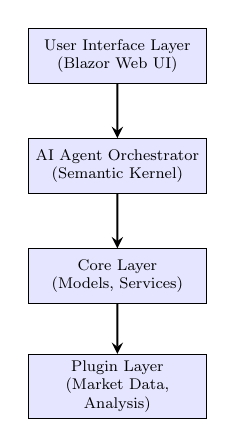
\begin{tikzpicture}[node distance=2cm, auto, scale=0.7, transform shape]
    % Define styles
    \tikzstyle{box}=[rectangle, draw=black, fill=blue!10, text width=3cm, text centered, minimum height=1cm, font=\footnotesize]
    \tikzstyle{arrow}=[->, thick, >=stealth]

    % Core layers
    \node[box] (ui) {User Interface Layer\\(Blazor Web UI)};
    \node[box] (orchestrator) [below of=ui] {AI Agent Orchestrator\\(Semantic Kernel)};
    \node[box] (core) [below of=orchestrator] {Core Layer\\(Models, Services)};
    \node[box] (plugins) [below of=core] {Plugin Layer\\(Market Data, Analysis)};

    % Connections
    \draw[arrow] (ui) -- (orchestrator);
    \draw[arrow] (orchestrator) -- (core);
    \draw[arrow] (core) -- (plugins);
\end{tikzpicture}
\caption{System Architecture Overview demonstrating the layered structure from presentation to data processing}
\label{fig:architecture}
\end{figure}


\subsection{Technology Stack}

\subsubsection{Core Technologies}
\begin{itemize}
    \item \textbf{Runtime}: .NET 9.0 with C\# 12.0
    \item \textbf{AI Framework}: Microsoft Semantic Kernel 1.25.0
    \item \textbf{LLM Integration}: OpenAI GPT-4, DeepSeek, and routing services
    \item \textbf{Mathematical Computing}: MathNet.Numerics, Microsoft.ML
    \item \textbf{Data Processing}: CsvHelper, System.Text.Json
\end{itemize}

\subsubsection{External Integrations}
\begin{itemize}
    \item \textbf{Brokerage}: Alpaca Markets API for trading execution
    \item \textbf{Market Data}: Polygon.io, Yahoo Finance, Alpha Vantage
    \item \textbf{News Sources}: Finviz, YFinance News, Reddit scraping
    \item \textbf{Economic Data}: FRED, World Bank, IMF, OECD
    \item \textbf{Academic Research}: Integration with research paper databases
\end{itemize}

\begin{figure}[htbp]
\centering
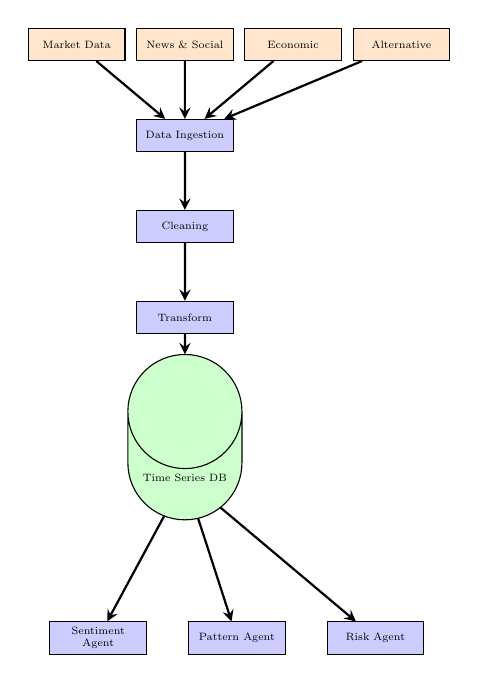
\begin{tikzpicture}[node distance=1.5cm, auto, scale=0.55, transform shape]
    \tikzstyle{source}=[rectangle, draw=black, fill=orange!20, text width=2cm, text centered, minimum height=0.75cm, font=\scriptsize]
    \tikzstyle{process}=[rectangle, draw=black, fill=blue!20, text width=2cm, text centered, minimum height=0.75cm, font=\scriptsize]
    \tikzstyle{storage}=[cylinder, draw=black, fill=green!20, text width=2.4cm, text centered, minimum height=0.9cm, font=\scriptsize, shape border rotate=90]
    \tikzstyle{arrow}=[->, thick, >=stealth]

    % Data sources
    \node[source] (market) {Market Data};
    \node[source] (news) [right of=market, xshift=1cm] {News \& Social};
    \node[source] (econ) [right of=news, xshift=1cm] {Economic};
    \node[source] (alt) [right of=econ, xshift=1cm] {Alternative};

    % Processing layer
    \node[process] (ingest) [below of=news, yshift=-0.6cm] {Data Ingestion};
    \node[process] (clean) [below of=ingest, yshift=-0.6cm] {Cleaning};
    \node[process] (transform) [below of=clean, yshift=-0.6cm] {Transform};

    % Storage
    \node[storage] (db) [below of=transform, yshift=-2.2cm] {Time Series DB};

    % Analysis layer
    \node[process] (agent1) [below of=db, yshift=-2.2cm, xshift=-2cm] {Sentiment Agent};
    \node[process] (agent2) [right of=agent1, xshift=1.7cm] {Pattern Agent};
    \node[process] (agent3) [right of=agent2, xshift=1.7cm] {Risk Agent};

    % Arrows
    \draw[arrow] (market) -- (ingest);
    \draw[arrow] (news) -- (ingest);
    \draw[arrow] (econ) -- (ingest);
    \draw[arrow] (alt) -- (ingest);
    \draw[arrow] (ingest) -- (clean);
    \draw[arrow] (clean) -- (transform);
    \draw[arrow] (transform) -- (db);
    \draw[arrow] (db) -- (agent1);
    \draw[arrow] (db) -- (agent2);
    \draw[arrow] (db) -- (agent3);
\end{tikzpicture}
\caption{Data Integration and Processing Flow demonstrating multi-source data pipeline from ingestion to agent analysis}
\label{fig:dataflow}
\end{figure}

\section{Current Capabilities}



\subsection{Core Research Agents}

FeenQR's agent orchestration system coordinates multiple specialized agents through the Semantic Kernel framework, enabling sophisticated multi-agent research workflows.

\begin{figure}[htbp]
\centering
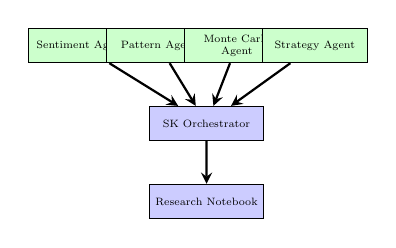
\begin{tikzpicture}[node distance=1.8cm, auto, scale=0.55, transform shape]
    % Define styles
    \tikzstyle{agent}=[rectangle, draw=black, fill=green!20, text width=2.2cm, text centered, minimum height=0.8cm, font=\scriptsize]
    \tikzstyle{process}=[rectangle, draw=black, fill=blue!20, text width=2.4cm, text centered, minimum height=0.8cm, font=\scriptsize]
    \tikzstyle{arrow}=[->, thick, >=stealth]

    % Agents
    \node[agent] (sentiment) {Sentiment Agent};
    \node[agent] (pattern) [right of=sentiment] {Pattern Agent};
    \node[agent] (montecarlo) [right of=pattern] {Monte Carlo Agent};
    \node[agent] (strategy) [right of=montecarlo] {Strategy Agent};

    % Orchestrator
    \node[process] (orchestrator) [below of=pattern, xshift=1.1cm] {SK Orchestrator};

    % Notebook
    \node[process] (notebook) [below of=orchestrator] {Research Notebook};

    % Connections
    \draw[arrow] (sentiment) -- (orchestrator);
    \draw[arrow] (pattern) -- (orchestrator);
    \draw[arrow] (montecarlo) -- (orchestrator);
    \draw[arrow] (strategy) -- (orchestrator);
    \draw[arrow] (orchestrator) -- (notebook);
\end{tikzpicture}
\caption{AI Agent Orchestration Workflow demonstrating multi-agent coordination through Semantic Kernel for autonomous research execution}
\label{fig:orchestration}
\end{figure}

\subsubsection{Market Sentiment Agent}
\textbf{Multi-Source Sentiment Analysis and Prediction}

The Market Sentiment Agent provides comprehensive sentiment analysis across multiple data sources:

\begin{itemize}
    \item \textbf{Financial News Analysis}: Real-time sentiment extraction from financial news
    \item \textbf{Social Media Monitoring}: Twitter, Reddit, and Discord sentiment aggregation
    \item \textbf{Fear \& Greed Index}: Integration with market sentiment indicators
    \item \textbf{Technical Sentiment}: Price action and volume-based sentiment signals
    \item \textbf{Market Direction Prediction}: AI-driven directional forecasting
\end{itemize}

\textbf{Key Features:}
\begin{itemize}
    \item Real-time sentiment aggregation with confidence weighting
    \item Contrarian vs. momentum signal generation
    \item Extreme sentiment alert systems
    \item Historical sentiment trend analysis
    \item Cross-asset sentiment correlation analysis
\end{itemize}

\begin{algorithm}[htbp]
\caption{Multi-Source Sentiment Aggregation}
\begin{algorithmic}[1]
\Require News articles $N$, social media posts $S$, technical indicators $T$
\Ensure Composite sentiment score $\in [-1, 1]$
\For{each news article $n \in N$}
    \State Extract entities and topics
    \State Calculate NLP sentiment: $s_n \in [-1, 1]$
    \State Assign source weight: $w_n$ based on credibility
\EndFor
\State Aggregate news sentiment: $S_{news} = \frac{\sum(w_n \cdot s_n)}{\sum(w_n)}$
\State Similarly calculate $S_{social}$ and $S_{technical}$
\State Apply source weights: $Composite = \alpha \cdot S_{news} + \beta \cdot S_{social} + \gamma \cdot S_{technical}$
\State Normalize to $[-1, 1]$ range
\If{$Composite > 0.3$}
    \State \Return BUY signal
\ElsIf{$Composite < -0.3$}
    \State \Return SELL signal
\Else
    \State \Return NEUTRAL signal
\EndIf
\end{algorithmic}
\end{algorithm}



\subsubsection{Statistical Pattern Agent}
\textbf{Deep Mathematical Market Analysis}

The Statistical Pattern Agent performs sophisticated mathematical analysis to detect exploitable market patterns:

\begin{itemize}
    \item \textbf{Mean Reversion Detection}: ADF tests, Hurst exponent analysis
    \item \textbf{Momentum Analysis}: Autocorrelation and trend strength measurement
    \item \textbf{Seasonal Effects}: Intraday, day-of-week, and monthly pattern analysis
    \item \textbf{Volatility Clustering}: GARCH modeling and volatility analysis
    \item \textbf{Statistical Anomalies}: Outlier detection and jump identification
\end{itemize}

\textbf{Supported Pattern Types:}
\begin{itemize}
    \item Mean reversion with statistical significance testing
    \item Momentum and trend pattern identification
    \item Seasonal and calendar effect analysis
    \item Volatility clustering and regime detection
    \item Correlation breakdown analysis
    \item Fractal patterns and self-similarity
    \item Arbitrage opportunity identification
    \item Market microstructure analysis
\end{itemize}

\begin{algorithm}[htbp]
\caption{Statistical Mean Reversion Detection}
\begin{algorithmic}[1]
\Require Price series $P$, lookback window $w$
\Ensure Mean reversion score and trading signal
\State Calculate log returns: $r[t] = \ln(P[t]/P[t-1])$
\State Perform ADF test for stationarity:
\State \quad $H_0$: Unit root (non-stationary)
\State \quad $H_1$: Stationary (mean reverting)
\State Calculate Hurst exponent $H$:
\If{$H < 0.5$}
    \State Pattern is mean reverting
\ElsIf{$H = 0.5$}
    \State Pattern is random walk
\Else
    \State Pattern is trending
\EndIf
\State Compute half-life of mean reversion:
\State Fit AR(1): $r[t] = \phi \cdot r[t-1] + \epsilon$
\State Half-life $= -\ln(2) / \ln(\phi)$
\State Calculate z-score: $z = (P - MA(w)) / \sigma(w)$
\If{$z < -2$}
    \State \Return BUY signal
\ElsIf{$z > 2$}
    \State \Return SELL signal
\Else
    \State \Return NEUTRAL signal
\EndIf
\end{algorithmic}
\end{algorithm}

\subsection{Research and Strategy Development Tools}

\subsubsection{Monte Carlo Simulation Framework}
\textbf{Advanced Risk Modeling and Scenario Analysis}

The Monte Carlo framework provides stochastic scenario generation for comprehensive risk assessment:

\begin{itemize}
    \item \textbf{Geometric Brownian Motion}: Price path simulation
    \item \textbf{Value-at-Risk Calculation}: Confidence interval-based risk metrics
    \item \textbf{Stress Testing}: Extreme market condition analysis
    \item \textbf{Probability Distributions}: Return and drawdown distribution analysis
\end{itemize}

\textbf{Key Capabilities:}
\begin{itemize}
    \item Customizable simulation parameters (horizon, volatility, drift)
    \item Multi-asset portfolio simulation
    \item Historical backtesting integration
    \item Risk metric calculations (VaR, CVaR, Expected Shortfall)
    \item Interactive visualization of simulation results
\end{itemize}

\begin{algorithm}[htbp]
\caption{Monte Carlo Price Path Simulation}
\begin{algorithmic}[1]
\Require Initial price $S_0$, drift $\mu$, volatility $\sigma$, time horizon $T$, simulations $N$
\Ensure Simulated price paths and risk metrics
\For{$i = 1$ to $N$}
    \State Initialize price path: $P[0] \gets S_0$
    \For{$t = 1$ to $T$}
        \State Generate random shock: $\epsilon \sim \mathcal{N}(0,1)$
        \State Compute return: $r = \mu \cdot \Delta t + \sigma \cdot \sqrt{\Delta t} \cdot \epsilon$
        \State Update price: $P[t] \gets P[t-1] \cdot \exp(r)$
    \EndFor
    \State Store final price: $S_{final}[i] \gets P[T]$
\EndFor
\State Calculate risk metrics:
\State \quad $VaR = Percentile(S_{final} - S_0, 5\%)$
\State \quad $CVaR = Mean(\text{losses below VaR})$
\State \Return price distribution and metrics
\end{algorithmic}
\end{algorithm}

\begin{figure}[htbp]
\centering
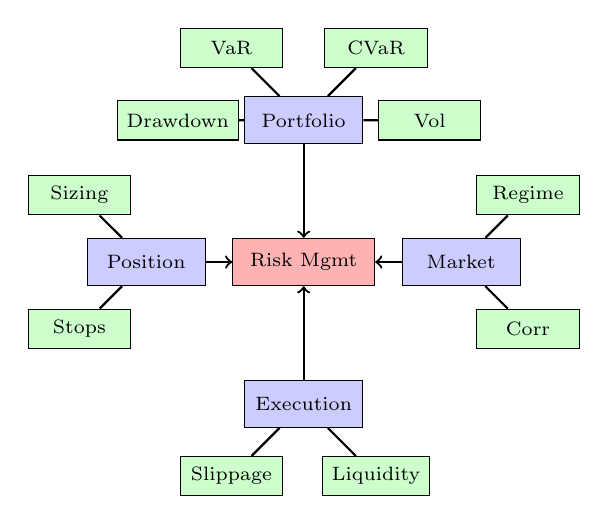
\begin{tikzpicture}[scale=0.38, node distance=1cm,
    box/.style={rectangle, draw, fill=blue!20, minimum width=1.5cm, minimum height=0.6cm, text centered, font=\scriptsize},
    metric/.style={rectangle, draw, fill=green!20, minimum width=1.3cm, minimum height=0.5cm, text centered, font=\scriptsize}]

% Central risk management node
\node[box, fill=red!30, minimum width=1.8cm] (center) {Risk Mgmt};

% Portfolio-level risks (top)
\node[box, above of=center, node distance=1.8cm] (portfolio) {Portfolio};
\node[metric, above left of=portfolio, node distance=1.3cm] (var) {VaR};
\node[metric, above right of=portfolio, node distance=1.3cm] (cvar) {CVaR};
\node[metric, left of=portfolio, node distance=1.6cm] (drawdown) {Drawdown};
\node[metric, right of=portfolio, node distance=1.6cm] (volatility) {Vol};

% Position-level risks (left)
\node[box, left of=center, node distance=2cm] (position) {Position};
\node[metric, above left of=position, node distance=1.2cm] (size) {Sizing};
\node[metric, below left of=position, node distance=1.2cm] (stops) {Stops};

% Market risks (right)
\node[box, right of=center, node distance=2cm] (market) {Market};
\node[metric, above right of=market, node distance=1.2cm] (regime) {Regime};
\node[metric, below right of=market, node distance=1.2cm] (correlation) {Corr};

% Execution risks (bottom)
\node[box, below of=center, node distance=1.8cm] (execution) {Execution};
\node[metric, below left of=execution, node distance=1.3cm] (slippage) {Slippage};
\node[metric, below right of=execution, node distance=1.3cm] (liquidity) {Liquidity};

% Connections
\draw[->, thick] (portfolio) -- (center);
\draw[->, thick] (position) -- (center);
\draw[->, thick] (market) -- (center);
\draw[->, thick] (execution) -- (center);

\draw[-, thick] (var) -- (portfolio);
\draw[-, thick] (cvar) -- (portfolio);
\draw[-, thick] (drawdown) -- (portfolio);
\draw[-, thick] (volatility) -- (portfolio);
\draw[-, thick] (size) -- (position);
\draw[-, thick] (stops) -- (position);
\draw[-, thick] (regime) -- (market);
\draw[-, thick] (correlation) -- (market);
\draw[-, thick] (slippage) -- (execution);
\draw[-, thick] (liquidity) -- (execution);

\end{tikzpicture}
\caption{Multi-Layer Risk Management Framework}
\label{fig:risk-framework}
\end{figure}

\subsubsection{Interactive Strategy Builder}
\textbf{Dynamic Trading Strategy Development}

The Strategy Builder provides visual strategy construction with real-time validation:

\begin{itemize}
    \item \textbf{Component-Based Design}: Drag-and-drop strategy construction
    \item \textbf{Real-Time Backtesting}: Historical performance validation
    \item \textbf{Parameter Optimization}: Genetic algorithm-based optimization
    \item \textbf{Walk-Forward Analysis}: Strategy robustness testing
\end{itemize}

\textbf{Strategy Components:}
\begin{itemize}
    \item Entry signals (technical indicators, patterns, volume analysis)
    \item Exit rules (profit targets, stop losses, trailing stops)
    \item Risk management (position sizing, portfolio heat)
    \item Filters (regime, volatility, correlation filters)
    \item Performance metrics (Sharpe, Sortino, maximum drawdown)
\end{itemize}

\begin{algorithm}[htbp]
\caption{Genetic Algorithm Strategy Optimization}
\begin{algorithmic}[1]
\Require Initial strategy $S$, parameter bounds, population size $P$, generations $G$
\Ensure Optimized strategy parameters
\State Initialize population of $P$ random strategies
\For{$gen = 1$ to $G$}
    \For{each strategy in population}
        \State Backtest strategy on historical data
        \State Calculate fitness $= f(Sharpe, Drawdown, WinRate, ProfitFactor)$
    \EndFor
    \State Select top 20\% strategies (elites)
    \State Create offspring via crossover:
    \State \quad Combine parameters from parent strategies
    \State Apply mutation: Randomly modify parameters
    \State Replace population with elites + offspring
\EndFor
\State \Return best performing strategy
\end{algorithmic}
\end{algorithm}

\subsubsection{Research Notebook Environment}
\textbf{Interactive Quantitative Research Platform}

The notebook environment provides a Jupyter-like interface for financial analysis:

\begin{itemize}
    \item \textbf{Code Execution}: Real-time code execution with output visualization
    \item \textbf{Markdown Support}: Documentation and analysis note integration
    \item \textbf{Service Integration}: Access to all FeenQR services and plugins
    \item \textbf{Export Capabilities}: Research finding documentation and sharing
\end{itemize}

\textbf{Built-in Analysis Tools:}
\begin{itemize}
    \item Data visualization (charts, graphs, statistical plots)
    \item Statistical analysis (hypothesis testing, regression)
    \item Time series analysis (ARIMA, GARCH, cointegration)
    \item Machine learning workflows (model training, evaluation)
    \item Performance analytics (benchmarking, comparison)
\end{itemize}

\begin{figure}[htbp]
\centering
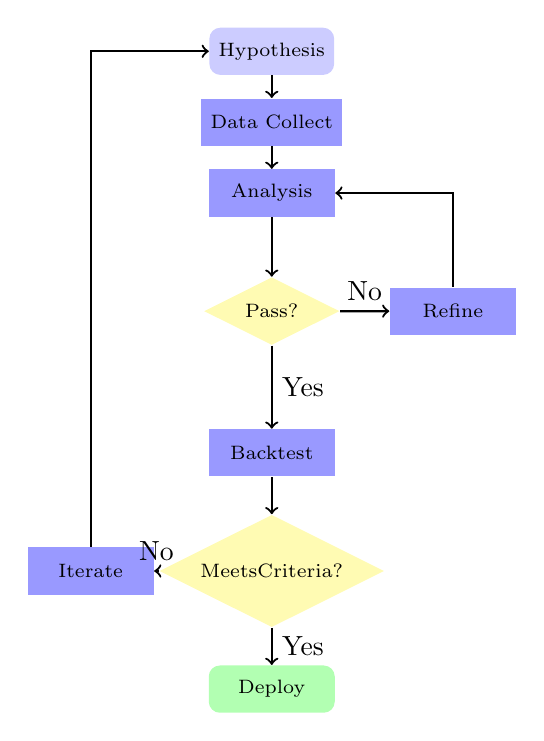
\begin{tikzpicture}[scale=0.42, node distance=0.9cm,
    start/.style={rectangle, rounded corners, fill=blue!20, minimum width=1.5cm, minimum height=0.6cm, text centered, font=\scriptsize},
    process/.style={rectangle, fill=blue!40, minimum width=1.6cm, minimum height=0.6cm, text centered, font=\scriptsize},
    decision/.style={diamond, fill=yellow!30, minimum width=1.4cm, minimum height=0.8cm, text centered, aspect=2, font=\scriptsize},
    result/.style={rectangle, rounded corners, fill=green!30, minimum width=1.6cm, minimum height=0.6cm, text centered, font=\scriptsize}]

% Workflow nodes
\node[start] (hypothesis) {Hypothesis};
\node[process, below of=hypothesis] (data) {Data Collect};
\node[process, below of=data] (analysis) {Analysis};
\node[decision, below of=analysis, node distance=1.5cm] (validate) {Pass?};
\node[process, right of=validate, node distance=2.3cm] (refine) {Refine};
\node[process, below of=validate, node distance=1.8cm] (backtest) {Backtest};
\node[decision, below of=backtest, node distance=1.5cm] (performance) {Meets\\Criteria?};
\node[result, below of=performance, node distance=1.5cm] (deploy) {Deploy};
\node[process, left of=performance, node distance=2.3cm] (iterate) {Iterate};

% Arrows
\draw[->, thick] (hypothesis) -- (data);
\draw[->, thick] (data) -- (analysis);
\draw[->, thick] (analysis) -- (validate);
\draw[->, thick] (validate) -- node[above] {No} (refine);
\draw[->, thick] (refine) |- (analysis);
\draw[->, thick] (validate) -- node[right] {Yes} (backtest);
\draw[->, thick] (backtest) -- (performance);
\draw[->, thick] (performance) -- node[right] {Yes} (deploy);
\draw[->, thick] (performance) -- node[above] {No} (iterate);
\draw[->, thick] (iterate) |- (hypothesis);

\end{tikzpicture}
\caption{Quantitative Research Workflow in Notebook Environment}
\label{fig:research-workflow}
\end{figure}

\subsection{Data Integration and Processing}

\subsubsection{Market Data Services}

\textbf{Multi-Vendor Market Data Integration}

FeenQR integrates with 15+ market data providers for comprehensive coverage:

\begin{itemize}
    \item \textbf{Alpaca Markets}: Commission-free stock and crypto trading API
    \item \textbf{Polygon.io}: Real-time and historical equities, options, forex, crypto
    \item \textbf{Alpha Vantage}: Technical indicators, fundamentals, forex, crypto
    \item \textbf{Yahoo Finance}: Free historical data and real-time quotes
    \item \textbf{IEX Cloud}: Real-time stock market data with enterprise features
    \item \textbf{Databento}: Institutional-grade tick data and normalized market data
    \item \textbf{Binance}: Cryptocurrency exchange data with WebSocket feeds
\end{itemize}

\textbf{Economic and Fundamental Data:}
\begin{itemize}
    \item \textbf{FRED (Federal Reserve)}: 800,000+ economic time series
    \item \textbf{World Bank}: Global development indicators and statistics
    \item \textbf{IMF}: International economic and financial data
    \item \textbf{OECD}: Organization for Economic Co-operation data
    \item \textbf{SEC Edgar}: Company filings (10-K, 10-Q, 8-K, proxy statements)
    \item \textbf{Financial Modeling Prep}: Financial statements and key metrics
    \item \textbf{Earnings Call Transcripts}: Automated extraction and NLP analysis
\end{itemize}

\subsection{Complete Plugin Ecosystem (80+ Plugins)}

\subsubsection{Market Data and Analysis Plugins}

\textbf{Technical Analysis Suite}
\begin{itemize}
    \item 150+ technical indicators (RSI, MACD, Bollinger Bands, Ichimoku)
    \item Chart pattern recognition (head-and-shoulders, triangles, flags)
    \item Support/resistance level identification
    \item Fibonacci retracement and extension analysis
    \item Elliott Wave theory implementation
    \item Candlestick pattern detection (50+ patterns)
\end{itemize}

\textbf{Fundamental Analysis Plugins}
\begin{itemize}
    \item \textbf{CompanyValuationPlugin}: DCF, DDM, comparable company analysis
    \item \textbf{EnhancedFundamentalAnalysisPlugin}: Balance sheet, income statement, cash flow analysis
    \item \textbf{EarningsAnalysisPlugin}: EPS trends, earnings surprise, guidance analysis
    \item \textbf{SECAnalysisPlugin}: 10-K/10-Q parsing and ratio calculations
    \item \textbf{CorporateActionPlugin}: Dividends, splits, M\&A event processing
\end{itemize}

\subsubsection{Alternative Data Plugins}

\textbf{News and Sentiment Analysis}
\begin{itemize}
    \item \textbf{MarketSentimentNewsPlugin}: Real-time news sentiment from 50+ sources
    \item \textbf{RedditFinancePlugin}: r/wallstreetbets, r/stocks sentiment analysis
    \item \textbf{WebIntelligencePlugin}: Web scraping for proprietary signals
    \item \textbf{YouTubeAnalysisPlugin}: Financial video content extraction
    \item \textbf{PodcastAnalysisPlugin}: Expert opinion aggregation from podcasts
\end{itemize}

\textbf{Advanced Alternative Data}
\begin{itemize}
    \item \textbf{SatelliteImageryAnalysisPlugin}: Retail parking lot analysis, shipping activity
    \item \textbf{SupplyChainPlugin}: Logistics patterns and inventory tracking
    \item \textbf{PatentAnalysisPlugin}: Technology trends from patent filings
    \item \textbf{GeopoliticalRiskPlugin}: Political risk scoring and event detection
\end{itemize}

\subsubsection{Quantitative Research Plugins}

\textbf{Statistical and Time Series Analysis}
\begin{itemize}
    \item \textbf{StatisticalTestingPlugin}: t-tests, ANOVA, chi-square, Kolmogorov-Smirnov
    \item \textbf{TimeSeriesAnalysisPlugin}: ARIMA, SARIMA, exponential smoothing
    \item \textbf{CointegrationPlugin}: Engle-Granger, Johansen, pairs trading
    \item \textbf{AnomalyDetectionPlugin}: Isolation forests, DBSCAN, autoencoders
    \item \textbf{FeatureEngineeringPlugin}: Automated feature generation and selection
\end{itemize}

\textbf{Advanced Modeling Plugins}
\begin{itemize}
    \item \textbf{FactorModelPlugin}: Fama-French 3/5/6 factor models, PCA
    \item \textbf{DynamicFactorPlugin}: Time-varying factor loadings
    \item \textbf{ForecastingPlugin}: Prophet, LSTM, GRU time series forecasting
    \item \textbf{AutoMLPlugin}: Automated model selection and hyperparameter tuning
    \item \textbf{ModelInterpretabilityPlugin}: SHAP values, LIME, feature importance
\end{itemize}

\subsubsection{Trading and Execution Plugins}

\textbf{Strategy Development}
\begin{itemize}
    \item \textbf{StrategyBuilderPlugin}: Visual strategy construction interface
    \item \textbf{TradingStrategyLibraryPlugin}: 50+ pre-built strategy templates
    \item \textbf{TradingTemplateGeneratorPlugin}: AI-powered strategy generation
    \item \textbf{EventDrivenTradingPlugin}: News-based and earnings-driven strategies
    \item \textbf{VolatilityTradingPlugin}: VIX trading, volatility arbitrage
    \item \textbf{OptionsFlowPlugin}: Unusual options activity detection
\end{itemize}

\textbf{Execution and Market Microstructure}
\begin{itemize}
    \item \textbf{ExecutionPlugin}: Smart order routing, TWAP/VWAP algorithms
    \item \textbf{FIXPlugin}: FIX protocol integration for institutional trading
    \item \textbf{HighFrequencyDataPlugin}: Tick-level analysis, order book dynamics
    \item \textbf{OrderBookPlugin}: Level II data analysis, liquidity measurement
    \item \textbf{LatencyArbitragePlugin}: Cross-exchange timing opportunities
    \item \textbf{MarketImpactPlugin}: Transaction cost analysis
\end{itemize}

\subsubsection{Risk Management Plugins}

\textbf{Portfolio Risk Analysis}
\begin{itemize}
    \item \textbf{RiskManagementPlugin}: VaR, CVaR, Expected Shortfall calculations
    \item \textbf{AdvancedRiskPlugin}: Stress testing, scenario analysis
    \item \textbf{AdvancedRiskAnalyticsPlugin}: Risk decomposition, marginal VaR
    \item \textbf{CounterpartyRiskPlugin}: Credit risk assessment
    \item \textbf{MarketRegimePlugin}: Regime detection (bull, bear, sideways)
\end{itemize}

\textbf{Performance and Attribution}
\begin{itemize}
    \item \textbf{PerformanceAttributionPlugin}: Factor-based return attribution
    \item \textbf{BenchmarkingPlugin}: Strategy comparison vs. indices
    \item \textbf{ComplianceMonitoringPlugin}: Real-time compliance checks
    \item \textbf{AutomatedReportingPlugin}: Daily/monthly performance reports
\end{itemize}

\subsubsection{Machine Learning Plugins}

\textbf{Advanced ML Frameworks}
\begin{itemize}
    \item \textbf{ReinforcementLearningPlugin}: Q-Learning, DQN, PPO for trading
    \item \textbf{AutoMLPlugin}: Automated model discovery and optimization
    \item \textbf{ModelValidationPlugin}: Walk-forward, purged cross-validation
    \item \textbf{FeatureEngineeringPlugin}: Automated feature creation
\end{itemize}

\subsubsection{Economic and Macro Plugins}

\textbf{Macroeconomic Analysis}
\begin{itemize}
    \item \textbf{FREDEconomicPlugin}: Federal Reserve economic data
    \item \textbf{FederalReservePlugin}: FOMC minutes, rate decision analysis
    \item \textbf{GlobalEconomicPlugin}: International economic indicators
    \item \textbf{IMFEconomicPlugin}: IMF World Economic Outlook data
    \item \textbf{OECEconomicPlugin}: OECD economic statistics
    \item \textbf{WorldBankEconomicPlugin}: World Bank development indicators
\end{itemize}

\subsubsection{Specialized Research Plugins}

\textbf{Academic and Industry Research}
\begin{itemize}
    \item \textbf{AcademicResearchPlugin}: arXiv, SSRN paper search and extraction
    \item \textbf{FactorResearchPlugin}: Academic factor discovery and testing
    \item \textbf{ConversationalResearchPlugin}: AI-powered research assistant
    \item \textbf{GoogleWebSearchPlugin}: Web search for research augmentation
\end{itemize}

\subsubsection{Analysis Plugins}
The system provides extensive plugin-based analysis capabilities:

\begin{itemize}
    \item \textbf{Technical Analysis}: Complete indicator library and pattern recognition
    \item \textbf{Fundamental Analysis}: Company valuation and financial modeling
    \item \textbf{Risk Analytics}: Portfolio risk assessment and optimization
    \item \textbf{Statistical Testing}: Hypothesis testing and significance analysis
    \item \textbf{Machine Learning}: Feature engineering and model validation
\end{itemize}

\begin{figure}[htbp]
\centering
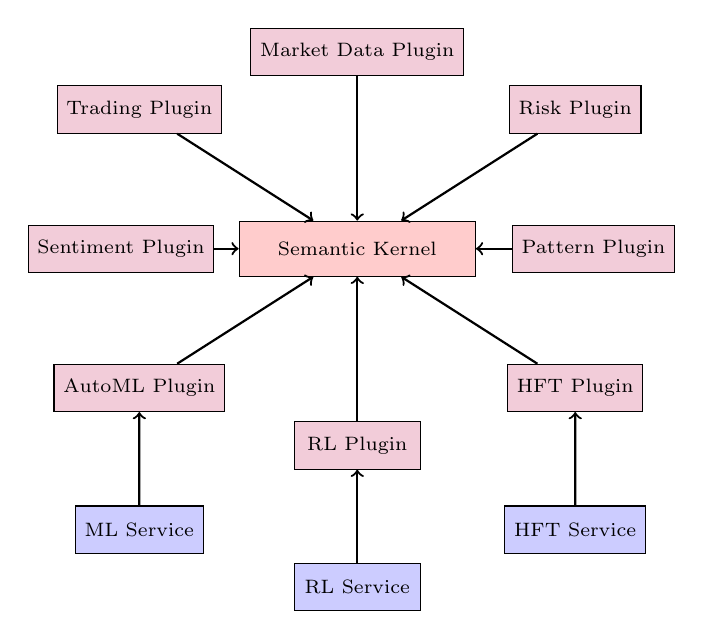
\begin{tikzpicture}[scale=0.38, node distance=1cm,
    plugin/.style={rectangle, draw, fill=purple!20, minimum width=1.6cm, minimum height=0.6cm, text centered, font=\scriptsize},
    service/.style={rectangle, draw, fill=blue!20, minimum width=1.6cm, minimum height=0.6cm, text centered, font=\scriptsize},
    core/.style={rectangle, draw, fill=red!20, minimum width=2.2cm, minimum height=0.7cm, text centered, font=\scriptsize}]

% Core Semantic Kernel
\node[core, minimum width=3cm] (kernel) {Semantic Kernel};

% Plugin categories
\node[plugin, above left of=kernel, node distance=2.5cm, xshift=-1cm] (trading) {Trading Plugin};
\node[plugin, above of=kernel, node distance=2.5cm] (market) {Market Data Plugin};
\node[plugin, above right of=kernel, node distance=2.5cm, xshift=1cm] (risk) {Risk Plugin};

\node[plugin, left of=kernel, node distance=3cm] (sentiment) {Sentiment Plugin};
\node[plugin, right of=kernel, node distance=3cm] (pattern) {Pattern Plugin};

\node[plugin, below left of=kernel, node distance=2.5cm, xshift=-1cm] (ml) {AutoML Plugin};
\node[plugin, below of=kernel, node distance=2.5cm] (rl) {RL Plugin};
\node[plugin, below right of=kernel, node distance=2.5cm, xshift=1cm] (hft) {HFT Plugin};

% Services backing plugins
\node[service, below of=ml, node distance=1.8cm] (mlsvc) {ML Service};
\node[service, below of=rl, node distance=1.8cm] (rlsvc) {RL Service};
\node[service, below of=hft, node distance=1.8cm] (hftsvc) {HFT Service};

% Connections
\draw[->, thick] (trading) -- (kernel);
\draw[->, thick] (market) -- (kernel);
\draw[->, thick] (risk) -- (kernel);
\draw[->, thick] (sentiment) -- (kernel);
\draw[->, thick] (pattern) -- (kernel);
\draw[->, thick] (ml) -- (kernel);
\draw[->, thick] (rl) -- (kernel);
\draw[->, thick] (hft) -- (kernel);

\draw[->, thick] (mlsvc) -- (ml);
\draw[->, thick] (rlsvc) -- (rl);
\draw[->, thick] (hftsvc) -- (hft);

\end{tikzpicture}
\caption{Plugin Architecture: Semantic Kernel orchestrates specialized plugins backed by domain services}
\label{fig:plugin-architecture}
\end{figure}

\subsection{Advanced Quantitative Capabilities}

\subsubsection{High-Frequency Trading and Market Microstructure}

\textbf{Market Microstructure Analysis}

FeenQR includes sophisticated high-frequency data analysis capabilities for institutional-grade trading strategies:

\begin{itemize}
    \item \textbf{Tick-Level Data Processing}: Sub-millisecond market data ingestion and analysis
    \item \textbf{Order Book Dynamics}: Level II data analysis for liquidity assessment
    \item \textbf{Hidden Order Detection}: AI-driven iceberg order and dark pool identification
    \item \textbf{Market Impact Modeling}: Transaction cost analysis and price impact prediction
    \item \textbf{Latency Arbitrage}: Cross-exchange timing opportunity detection
\end{itemize}

\textbf{Avellaneda-Stoikov Market Making}

The system implements advanced market making strategies:
\begin{itemize}
    \item Risk-averse optimal bid-ask spread calculation
    \item Dynamic inventory management with mean reversion
    \item Adverse selection protection mechanisms
    \item Real-time volatility adjustment of quotes
    \item PnL optimization under inventory constraints
\end{itemize}

\begin{figure}[htbp]
\centering
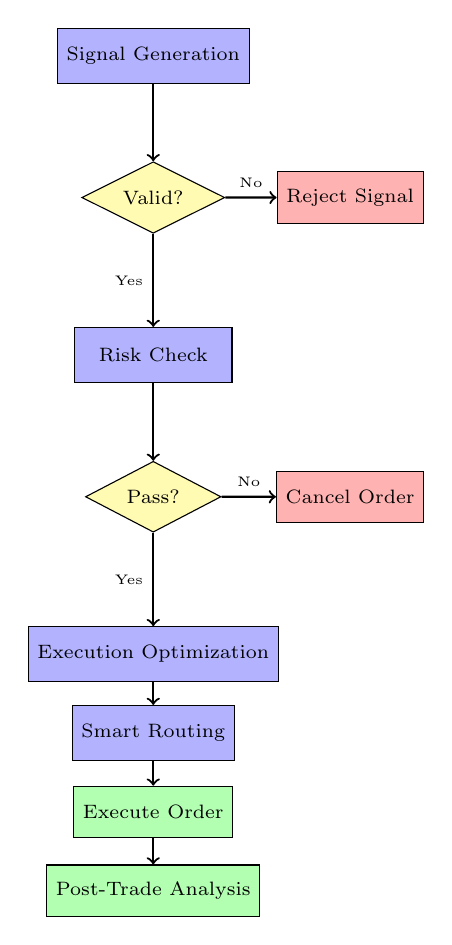
\begin{tikzpicture}[scale=0.38, node distance=1cm,
    stage/.style={rectangle, draw, fill=blue!30, minimum width=2cm, minimum height=0.7cm, text centered, font=\scriptsize},
    check/.style={diamond, draw, fill=yellow!30, minimum width=1.5cm, minimum height=0.9cm, text centered, font=\scriptsize, aspect=2},
    action/.style={rectangle, draw, fill=green!30, minimum width=1.8cm, minimum height=0.65cm, text centered, font=\scriptsize}]

% Pipeline stages
\node[stage] (signal) {Signal Generation};
\node[check, below of=signal, node distance=1.8cm] (validate) {Valid?};
\node[stage, below of=validate, node distance=2cm] (risk) {Risk Check};
\node[check, below of=risk, node distance=1.8cm] (pass) {Pass?};
\node[stage, below of=pass, node distance=2cm] (optimize) {Execution Optimization};
\node[stage, below of=optimize] (route) {Smart Routing};
\node[action, below of=route] (execute) {Execute Order};
\node[action, below of=execute] (monitor) {Post-Trade Analysis};

% Rejection paths
\node[action, right of=validate, node distance=2.5cm, fill=red!30] (reject1) {Reject Signal};
\node[action, right of=pass, node distance=2.5cm, fill=red!30] (reject2) {Cancel Order};

% Connections
\draw[->, thick] (signal) -- (validate);
\draw[->, thick] (validate) -- node[left, font=\tiny] {Yes} (risk);
\draw[->, thick] (validate) -- node[above, font=\tiny] {No} (reject1);
\draw[->, thick] (risk) -- (pass);
\draw[->, thick] (pass) -- node[left, font=\tiny] {Yes} (optimize);
\draw[->, thick] (pass) -- node[above, font=\tiny] {No} (reject2);
\draw[->, thick] (optimize) -- (route);
\draw[->, thick] (route) -- (execute);
\draw[->, thick] (execute) -- (monitor);

\end{tikzpicture}
\caption{Trading Execution Pipeline with multi-stage validation and optimization}
\label{fig:execution-pipeline}
\end{figure}

\subsubsection{Reinforcement Learning for Trading}

\textbf{Multi-Agent RL Framework}

State-of-the-art reinforcement learning capabilities for autonomous strategy discovery:

\begin{itemize}
    \item \textbf{Q-Learning Agents}: Discrete action space strategy optimization
    \item \textbf{Policy Gradient Methods}: Continuous action optimization (position sizing)
    \item \textbf{Actor-Critic Architecture}: Advanced RL with value function approximation
    \item \textbf{Deep Q-Networks (DQN)}: Neural network-based Q-function approximation
    \item \textbf{Proximal Policy Optimization}: Stable policy gradient optimization
    \item \textbf{Multi-Asset Coordination}: Portfolio-level RL strategy development
\end{itemize}

\textbf{Training Infrastructure:}
\begin{itemize}
    \item Parallel environment simulation for rapid training
    \item Experience replay buffer for sample efficiency
    \item Reward shaping for convergence acceleration
    \item Walk-forward validation with market regime adaptation
    \item Transfer learning across similar market instruments
\end{itemize}

\subsubsection{Factor Models and Risk Decomposition}

\textbf{Multi-Factor Risk Models}

Comprehensive factor modeling framework for portfolio construction and risk attribution:

\begin{itemize}
    \item \textbf{Fama-French Models}: 3-factor, 5-factor, and 6-factor implementations
    \item \textbf{Principal Component Analysis}: Data-driven factor extraction
    \item \textbf{Dynamic Factor Models}: Time-varying factor loadings and exposures
    \item \textbf{Industry and Sector Factors}: Customizable factor hierarchies
    \item \textbf{Style Factors}: Value, momentum, quality, low volatility, size
\end{itemize}

\textbf{Risk Decomposition:}
\begin{itemize}
    \item Factor contribution to portfolio variance
    \item Idiosyncratic vs. systematic risk separation
    \item Marginal contribution to risk (MCTR)
    \item Risk budgeting and allocation optimization
    \item Stress testing under factor shocks
\end{itemize}

\subsection{Services Layer Architecture (80+ Services)}

\subsubsection{Core Service Infrastructure}

\textbf{LLM and AI Services}

FeenQR implements sophisticated AI service orchestration:

\begin{itemize}
    \item \textbf{OpenAIService}: GPT-4, GPT-4-Turbo integration for analysis
    \item \textbf{DeepSeekService}: Alternative LLM for cost optimization
    \item \textbf{LLMRouterService}: Intelligent routing based on task complexity
    \item \textbf{IntelligentAIAssistantService}: Conversational research interface
\end{itemize}

\textbf{Market Data Services (15+ Providers)}

\begin{itemize}
    \item \textbf{AlpacaService / AdvancedAlpacaService}: Commission-free trading and market data
    \item \textbf{PolygonService}: Real-time and historical multi-asset data
    \item \textbf{AlphaVantageService}: Technical indicators and fundamental data
    \item \textbf{YahooFinanceService}: Free historical data provider
    \item \textbf{IEXCloudService}: Real-time stock market data
    \item \textbf{DataBentoService}: Institutional-grade normalized market data
    \item \textbf{MarketDataService}: Unified interface to all data providers
\end{itemize}

\subsubsection{Research Services}

\textbf{Academic and Quantitative Research}

\begin{itemize}
    \item \textbf{AcademicResearchService}: arXiv and SSRN paper search/extraction
    \item \textbf{FactorResearchService}: Factor discovery and backtesting
    \item \textbf{ConversationalResearchService}: AI-powered research assistant
    \item \textbf{NotebookService}: Interactive Jupyter-style research environment
    \item \textbf{StrategyGeneratorService}: AI-driven strategy synthesis
\end{itemize}

\textbf{Statistical and Time Series Services}

\begin{itemize}
    \item \textbf{StatisticalTestingService}: Comprehensive hypothesis testing suite
    \item \textbf{TimeSeriesAnalysisService}: ARIMA, GARCH, cointegration
    \item \textbf{TimeSeriesForecastingService}: Prophet, LSTM, GRU forecasting
    \item \textbf{CointegrationAnalysisService}: Pairs trading and statistical arbitrage
    \item \textbf{AnomalyDetectionService}: Outlier and regime change detection
\end{itemize}

\subsubsection{Alternative Data Services}

\textbf{News and Sentiment Services}

\begin{itemize}
    \item \textbf{NewsSentimentAnalysisService}: Multi-source sentiment aggregation
    \item \textbf{NewsScrapingService}: Automated news collection from 50+ sources
    \item \textbf{FinvizNewsService}: Real-time financial news scraping
    \item \textbf{YFinanceNewsService}: Yahoo Finance news integration
    \item \textbf{RealNewsService}: Verified news source filtering
\end{itemize}

\textbf{Social Media and Web Intelligence}

\begin{itemize}
    \item \textbf{RedditScrapingService}: Reddit financial community analysis
    \item \textbf{SocialMediaScrapingService}: Twitter, Discord sentiment
    \item \textbf{WebIntelligenceService}: Proprietary web signal extraction
    \item \textbf{WebDataExtractionService}: Structured data extraction
    \item \textbf{YouTubeAnalysisService}: Financial video content processing
\end{itemize}

\textbf{Advanced Alternative Data}

\begin{itemize}
    \item \textbf{RealSatelliteImageryService}: Parking lot, shipping activity analysis
    \item \textbf{SatelliteImageryAnalysisService}: Computer vision for retail tracking
    \item \textbf{SupplyChainService}: Logistics pattern analysis
    \item \textbf{PatentAnalysisService}: Technology trend identification
    \item \textbf{GeopoliticalRiskService}: Political risk scoring
\end{itemize}

\subsubsection{Trading and Execution Services}

\textbf{Strategy Development Services}

\begin{itemize}
    \item \textbf{StrategyBuilderService}: Visual strategy construction
    \item \textbf{TradingStrategyLibraryService}: 50+ pre-built strategies
    \item \textbf{LiveStrategyService}: Real-time strategy execution
    \item \textbf{EventDrivenTradingService}: News and earnings-based trading
    \item \textbf{VolatilityTradingService}: VIX and volatility arbitrage
\end{itemize}

\textbf{Execution and Microstructure Services}

\begin{itemize}
    \item \textbf{ExecutionService}: Smart order routing, TWAP/VWAP algorithms
    \item \textbf{FIXService}: FIX protocol for institutional connectivity
    \item \textbf{HighFrequencyDataService}: Tick-level analysis, market making
    \item \textbf{OrderBookAnalysisService}: Level II data analysis
    \item \textbf{LatencyArbitrageService}: Cross-exchange arbitrage
    \item \textbf{MarketImpactService}: Transaction cost analysis
    \item \textbf{OptionsFlowService}: Unusual options activity detection
\end{itemize}

\subsubsection{Risk and Portfolio Services}

\textbf{Risk Management Services}

\begin{itemize}
    \item \textbf{RiskManagementService}: VaR, CVaR, stress testing
    \item \textbf{AdvancedRiskService}: Scenario analysis, what-if simulations
    \item \textbf{AdvancedRiskAnalyticsService}: Risk decomposition, attribution
    \item \textbf{CounterpartyRiskService}: Credit risk assessment
    \item \textbf{MarketRegimeService}: Bull/bear/sideways regime detection
\end{itemize}

\textbf{Portfolio and Performance Services}

\begin{itemize}
    \item \textbf{PortfolioService}: Position tracking, PnL calculation
    \item \textbf{PortfolioOptimizationService}: Mean-variance, Black-Litterman
    \item \textbf{PerformanceAttributionService}: Factor-based attribution
    \item \textbf{BenchmarkingService}: Strategy vs. index comparison
    \item \textbf{ReportGenerationService}: Automated tear sheets
\end{itemize}

\subsubsection{Machine Learning Services}

\textbf{ML and AutoML Services}

\begin{itemize}
    \item \textbf{AutoMLService}: Automated model selection and tuning
    \item \textbf{ModelValidationService}: Walk-forward, purged CV
    \item \textbf{ModelInterpretabilityService}: SHAP, LIME, feature importance
    \item \textbf{FeatureEngineeringService}: Automated feature generation
    \item \textbf{ReinforcementLearningService}: Q-Learning, DQN, PPO agents
\end{itemize}

\subsubsection{Economic Data Services}

\textbf{Macroeconomic Services}

\begin{itemize}
    \item \textbf{FREDService}: 800,000+ Federal Reserve economic time series
    \item \textbf{FederalReserveService}: FOMC minutes, rate decisions
    \item \textbf{GlobalEconomicService}: International economic indicators
    \item \textbf{IMFService}: IMF World Economic Outlook data
    \item \textbf{OECDService}: OECD economic statistics
    \item \textbf{WorldBankService}: World Bank development indicators
\end{itemize}

\subsubsection{Fundamental Analysis Services}

\textbf{Company Analysis Services}

\begin{itemize}
    \item \textbf{CompanyValuationService}: DCF, DDM, comparable analysis
    \item \textbf{EnhancedFundamentalAnalysisService}: Financial statement analysis
    \item \textbf{EarningsCallService}: Earnings call transcript processing
    \item \textbf{SECFilingsService}: 10-K, 10-Q, 8-K automated parsing
    \item \textbf{CorporateActionService}: Dividend, split, M\&A tracking
    \item \textbf{FinancialModelingPrepService}: Financial metrics API
\end{itemize}

\subsubsection{Specialized Services}

\textbf{Advanced Quantitative Services}

\begin{itemize}
    \item \textbf{MonteCarloService}: Stochastic simulation and VaR
    \item \textbf{FactorModelService}: Multi-factor model implementation
    \item \textbf{DynamicFactorService}: Time-varying factor models
    \item \textbf{TechnicalAnalysisService}: 150+ technical indicators
    \item \textbf{AdvancedMicrostructureService}: Order flow analysis
    \item \textbf{AdvancedOptimizationService}: Portfolio optimization algorithms
\end{itemize}

\textbf{Operational Services}

\begin{itemize}
    \item \textbf{ComplianceMonitoringService}: Real-time compliance checks
    \item \textbf{RealTimeAlertingService}: Custom alert system
    \item \textbf{AutomatedReportingService}: Scheduled report generation
    \item \textbf{DataValidationService}: Data quality monitoring
    \item \textbf{TimezoneService}: Global timezone handling
\end{itemize}

\subsubsection{Alternative Data Integration}

\textbf{Multi-Source Alternative Data}

FeenQR integrates diverse alternative data sources for alpha generation:

\begin{itemize}
    \item \textbf{Satellite Imagery}: Supply chain monitoring and retail activity tracking
    \item \textbf{Web Traffic Analysis}: Company website visitor trends and engagement
    \item \textbf{Social Media Sentiment}: Twitter, Reddit, Discord financial discussions
    \item \textbf{News Analytics}: Real-time news sentiment and event detection
    \item \textbf{Patent Analysis}: Technology trend identification and innovation metrics
    \item \textbf{Supply Chain Data}: Logistics patterns and inventory tracking
    \item \textbf{Podcast/YouTube Analysis}: Expert opinion aggregation and theme extraction
\end{itemize}

\textbf{Data Processing Pipeline:}
\begin{itemize}
    \item Automated data collection with rate limiting and error handling
    \item Natural language processing for sentiment extraction
    \item Computer vision for satellite imagery analysis
    \item Time series alignment and resampling
    \item Predictive feature engineering from raw alternative data
    \item Signal generation with confidence scoring
\end{itemize}

\subsection{Compliance and Regulatory Features}

\subsubsection{Real-Time Compliance Monitoring}

\textbf{Automated Compliance Framework}

Built-in regulatory compliance capabilities for institutional deployment:

\begin{itemize}
    \item \textbf{Pre-Trade Risk Checks}: Position limits, concentration limits, leverage constraints
    \item \textbf{Best Execution Analysis}: VWAP/TWAP comparison and execution quality metrics
    \item \textbf{Market Manipulation Detection}: Wash trading, spoofing, layering detection
    \item \textbf{Audit Trail Generation}: Complete order lifecycle documentation
    \item \textbf{Regulatory Reporting}: MiFID II, SEC Rule 605, CAT reporting preparation
\end{itemize}

\subsubsection{Corporate Actions and Events}

\textbf{Corporate Event Management}

Comprehensive corporate action handling for accurate backtesting and live trading:

\begin{itemize}
    \item \textbf{Dividend Adjustments}: Ex-dividend date processing and yield calculations
    \item \textbf{Stock Splits}: Forward and reverse split adjustments
    \item \textbf{Mergers \& Acquisitions}: Symbol changes and cash/stock conversions
    \item \textbf{Earnings Events}: Earnings announcement detection and impact analysis
    \item \textbf{Spin-offs and Delistings}: Portfolio position adjustments
\end{itemize}

\subsection{Machine Learning and AutoML}

\subsubsection{Automated Machine Learning Pipeline}

\textbf{End-to-End AutoML Framework}

Sophisticated AutoML capabilities for model discovery and optimization:

\begin{itemize}
    \item \textbf{Algorithm Selection}: Automated model comparison (XGBoost, LightGBM, Random Forests, Neural Networks, SVMs)
    \item \textbf{Hyperparameter Tuning}: Bayesian optimization, grid search, random search, hyperband
    \item \textbf{Feature Selection}: Recursive feature elimination, Boruta, mutual information
    \item \textbf{Ensemble Construction}: Stacking, blending, voting ensembles with meta-learners
    \item \textbf{Model Interpretability}: SHAP values, LIME, partial dependence plots, feature importance
    \item \textbf{Online Learning}: Incremental model updates with concept drift detection
\end{itemize}

\textbf{Advanced ML Techniques:}
\begin{itemize}
    \item Neural architecture search for deep learning models
    \item Meta-learning for rapid adaptation to new markets
    \item Few-shot learning for limited data regimes
    \item Transfer learning across correlated assets
    \item Multi-task learning for related prediction problems
\end{itemize}

\textbf{Validation Framework:}
\begin{itemize}
    \item Walk-forward analysis with expanding/rolling windows
    \item Purged cross-validation for time series
    \item Combinatorial purged CV for overlapping data
    \item Out-of-sample testing with embargo periods
    \item Regime-aware validation splits
\end{itemize}

\subsection{Agent Orchestration and Workflow}

\subsubsection{Semantic Kernel Agent Framework}

\textbf{Multi-Agent Coordination Architecture}

FeenQR implements a sophisticated multi-agent system using Microsoft Semantic Kernel:

\begin{itemize}
    \item \textbf{Agent Specialization}: Each agent focuses on specific domain expertise
    \item \textbf{Hierarchical Orchestration}: Master orchestrator coordinates sub-agents
    \item \textbf{Message Passing}: Agents communicate via structured message protocols
    \item \textbf{Parallel Execution}: Independent agents run concurrently for efficiency
    \item \textbf{Result Aggregation}: Intelligent synthesis of multi-agent outputs
    \item \textbf{Conflict Resolution}: Voting and weighted consensus mechanisms
\end{itemize}

\textbf{Agent Lifecycle Management:}
\begin{itemize}
    \item Dynamic agent instantiation based on research goals
    \item Resource pooling and agent reuse for efficiency
    \item Graceful degradation when agents fail
    \item Agent performance monitoring and adaptive selection
    \item Historical agent decision tracking for accountability
\end{itemize}

\subsubsection{Complete Agent Roster}

\textbf{Research and Analysis Agents}
\begin{itemize}
    \item \textbf{Market Sentiment Agent}: Multi-source sentiment aggregation
    \item \textbf{Statistical Pattern Agent}: Mathematical pattern detection
    \item \textbf{Monte Carlo Agent}: Stochastic simulation and risk modeling
    \item \textbf{Strategy Builder Agent}: Automated strategy construction
    \item \textbf{Factor Analysis Agent}: Multi-factor model implementation
    \item \textbf{Cointegration Agent}: Statistical arbitrage identification
    \item \textbf{Volatility Agent}: Volatility forecasting and trading
    \item \textbf{Regime Detection Agent}: Market state classification
\end{itemize}

\textbf{Data Collection Agents}
\begin{itemize}
    \item \textbf{News Scraping Agent}: Multi-source news collection
    \item \textbf{Social Media Agent}: Reddit, Twitter sentiment extraction
    \item \textbf{Economic Data Agent}: FRED, World Bank, IMF data retrieval
    \item \textbf{Fundamental Data Agent}: SEC filings, financial statements
    \item \textbf{Alternative Data Agent}: Satellite, web traffic, patents
    \item \textbf{Market Data Agent}: Real-time and historical price data
\end{itemize}

\textbf{Execution and Risk Agents}
\begin{itemize}
    \item \textbf{Risk Management Agent}: Portfolio risk assessment
    \item \textbf{Execution Agent}: Smart order routing
    \item \textbf{Compliance Agent}: Real-time regulatory checks
    \item \textbf{Portfolio Optimization Agent}: Mean-variance optimization
    \item \textbf{Performance Attribution Agent}: Factor-based attribution
\end{itemize}

\subsubsection{Agent Communication Protocols}

\textbf{Inter-Agent Messaging}

Agents communicate using standardized message formats:

\begin{itemize}
    \item \textbf{JSON Schema Validation}: All messages validated against schemas
    \item \textbf{Semantic Message Types}: QUERY, RESPONSE, NOTIFICATION, ALERT
    \item \textbf{Priority Queues}: Urgent messages bypass normal queue
    \item \textbf{Message Persistence}: Critical messages stored for audit
    \item \textbf{Retry Logic}: Automatic retries with exponential backoff
\end{itemize}

\textbf{Agent Orchestration Patterns:}
\begin{itemize}
    \item \textbf{Sequential Pipeline}: Agents process data in stages
    \item \textbf{Parallel Broadcast}: Query sent to multiple agents simultaneously
    \item \textbf{Map-Reduce}: Distribute work, aggregate results
    \item \textbf{Conditional Routing}: Route to agents based on context
    \item \textbf{Feedback Loops}: Iterative refinement with agent collaboration
\end{itemize}

\subsection{Technical Implementation Details}

\subsubsection{Performance Optimization}

\textbf{High-Performance Computing Techniques}

FeenQR employs advanced optimization strategies:

\begin{itemize}
    \item \textbf{Async/Await Pattern}: Non-blocking I/O throughout codebase
    \item \textbf{Parallel.ForEach}: Multi-core CPU utilization
    \item \textbf{Memory Pooling}: Reduce GC pressure with object pooling
    \item \textbf{Span<T> and Memory<T>}: Zero-copy buffer operations
    \item \textbf{SIMD Vectorization}: Hardware-accelerated numerical operations
    \item \textbf{Caching Strategies}: Redis for distributed caching, in-memory for hot data
\end{itemize}

\textbf{Database Optimization:}
\begin{itemize}
    \item \textbf{TimescaleDB}: PostgreSQL extension for time series data
    \item \textbf{Hypertables}: Automatic partitioning by time
    \item \textbf{Continuous Aggregates}: Pre-computed rollups for fast queries
    \item \textbf{Compression}: Transparent time series compression
    \item \textbf{Connection Pooling}: Efficient database connection reuse
    \item \textbf{Prepared Statements}: Query plan caching
\end{itemize}

\subsubsection{Scalability Architecture}

\textbf{Horizontal Scaling Strategy}

Production deployment supports massive scale:

\begin{itemize}
    \item \textbf{Containerization}: Docker containers for each service
    \item \textbf{Kubernetes Orchestration}: Auto-scaling based on load
    \item \textbf{Load Balancing}: NGINX for traffic distribution
    \item \textbf{Service Mesh}: Istio for microservice communication
    \item \textbf{Message Queue}: RabbitMQ for asynchronous processing
    \item \textbf{Event Sourcing}: Complete audit trail of all events
\end{itemize}

\textbf{Resilience and Fault Tolerance:}
\begin{itemize}
    \item \textbf{Circuit Breakers}: Prevent cascade failures (Polly library)
    \item \textbf{Retry Policies}: Exponential backoff with jitter
    \item \textbf{Bulkhead Isolation}: Separate thread pools per service
    \item \textbf{Health Checks}: Kubernetes liveness and readiness probes
    \item \textbf{Graceful Degradation}: Fallback to cached data
    \item \textbf{Distributed Tracing}: OpenTelemetry for request tracking
\end{itemize}

\subsubsection{Security and Authentication}

\textbf{Enterprise Security Features}

\begin{itemize}
    \item \textbf{API Key Management}: Secure credential storage in Azure Key Vault
    \item \textbf{OAuth 2.0 / OpenID Connect}: Modern authentication flows
    \item \textbf{Role-Based Access Control}: Fine-grained permissions
    \item \textbf{Encryption}: TLS 1.3 for transit, AES-256 for rest
    \item \textbf{Audit Logging}: Comprehensive activity tracking
    \item \textbf{Rate Limiting}: API quota enforcement per user/key
    \item \textbf{SQL Injection Prevention}: Parameterized queries
    \item \textbf{CSRF Protection}: Anti-forgery tokens
\end{itemize}

Sophisticated AutoML capabilities for model discovery and optimization:

\begin{itemize}
    \item \textbf{Algorithm Selection}: Automated model comparison (XGBoost, LightGBM, Neural Nets)
    \item \textbf{Hyperparameter Tuning}: Bayesian optimization and grid search
    \item \textbf{Feature Selection}: Recursive feature elimination and importance ranking
    \item \textbf{Ensemble Construction}: Stacking, blending, and voting ensembles
    \item \textbf{Model Interpretability}: SHAP values and feature importance analysis
    \item \textbf{Online Learning}: Incremental model updates with new market data
\end{itemize}

\textbf{Validation Framework:}
\begin{itemize}
    \item Walk-forward analysis with expanding/rolling windows
    \item Purged cross-validation for time series
    \item Combinatorial purged CV for overlapping data
    \item Out-of-sample testing with embargo periods
    \item Regime-aware validation splits
\end{itemize}

\begin{figure}[htbp]
\centering
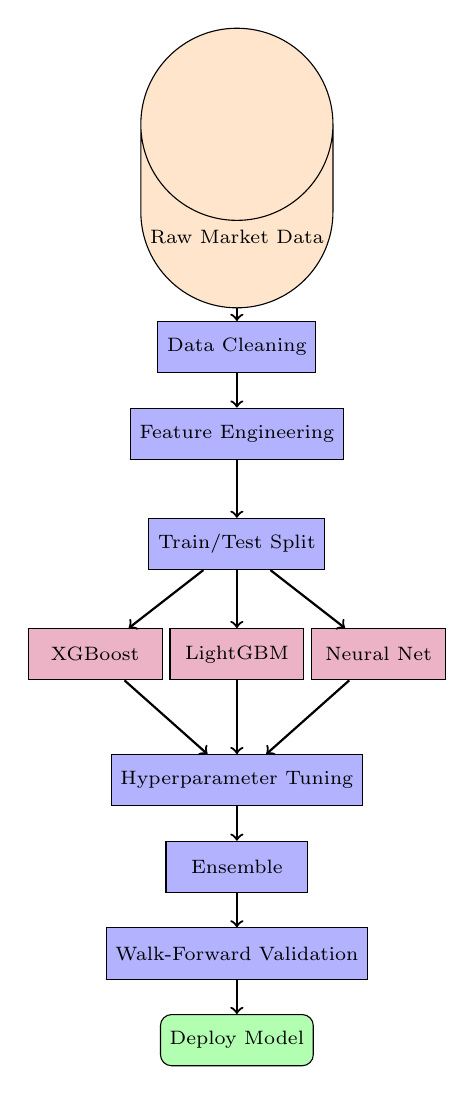
\begin{tikzpicture}[scale=0.38, node distance=1.1cm,
    data/.style={cylinder, draw, fill=orange!20, minimum width=1.5cm, minimum height=0.6cm, font=\scriptsize, shape border rotate=90},
    process/.style={rectangle, draw, fill=blue!30, minimum width=1.8cm, minimum height=0.65cm, text centered, font=\scriptsize},
    model/.style={rectangle, draw, fill=purple!30, minimum width=1.7cm, minimum height=0.65cm, text centered, font=\scriptsize},
    output/.style={rectangle, rounded corners, draw, fill=green!30, minimum width=1.8cm, minimum height=0.65cm, text centered, font=\scriptsize}]

% Data stage
\node[data] (rawdata) {Raw Market Data};
\node[process, below of=rawdata, yshift=-0.3cm] (clean) {Data Cleaning};
\node[process, below of=clean] (features) {Feature Engineering};

% Model training stage
\node[process, below of=features, yshift=-0.3cm] (split) {Train/Test Split};
\node[model, below of=split, yshift=-0.3cm, xshift=-1.8cm] (model1) {XGBoost};
\node[model, below of=split, yshift=-0.3cm] (model2) {LightGBM};
\node[model, below of=split, yshift=-0.3cm, xshift=1.8cm] (model3) {Neural Net};

% Optimization and ensemble
\node[process, below of=model2, yshift=-0.5cm] (optimize) {Hyperparameter Tuning};
\node[process, below of=optimize] (ensemble) {Ensemble};

% Validation and deployment
\node[process, below of=ensemble] (validate) {Walk-Forward Validation};
\node[output, below of=validate] (deploy) {Deploy Model};

% Connections
\draw[->, thick] (rawdata) -- (clean);
\draw[->, thick] (clean) -- (features);
\draw[->, thick] (features) -- (split);
\draw[->, thick] (split) -- (model1);
\draw[->, thick] (split) -- (model2);
\draw[->, thick] (split) -- (model3);
\draw[->, thick] (model1) -- (optimize);
\draw[->, thick] (model2) -- (optimize);
\draw[->, thick] (model3) -- (optimize);
\draw[->, thick] (optimize) -- (ensemble);
\draw[->, thick] (ensemble) -- (validate);
\draw[->, thick] (validate) -- (deploy);

\end{tikzpicture}
\caption{AutoML Pipeline: Automated model selection, optimization, and ensemble construction}
\label{fig:automl-pipeline}
\end{figure}

\subsection{Production Deployment Architecture}

\subsubsection{Blazor Web Interface}

\textbf{Bloomberg Terminal-Style Dashboard}

FeenQR includes a sophisticated web interface for professional quantitative research:

\begin{itemize}
    \item \textbf{Multi-Widget Dashboard}: Customizable layout with drag-and-drop widgets
    \item \textbf{Real-Time Data Streaming}: SignalR integration for live market updates
    \item \textbf{Interactive Charting}: TradingView-style charts with technical overlays
    \item \textbf{Portfolio Management}: Live position tracking and PnL monitoring
    \item \textbf{Research Notebook}: Browser-based Jupyter-style environment
    \item \textbf{Strategy Builder}: Visual strategy development interface
    \item \textbf{Alert Management}: Configurable real-time alert system
\end{itemize}

\textbf{Widget Library:}
\begin{itemize}
    \item Market Data Widget: Real-time quotes and depth of book
    \item Sentiment Dashboard: Multi-source sentiment aggregation
    \item Risk Monitor: Portfolio risk metrics and VaR tracking
    \item News Feed: Filtered financial news with sentiment scores
    \item Economic Calendar: Upcoming events and impact forecasts
    \item Backtesting Results: Strategy performance visualization
    \item Order Management: Trade execution and monitoring
\end{itemize}

\begin{figure}[htbp]
\centering
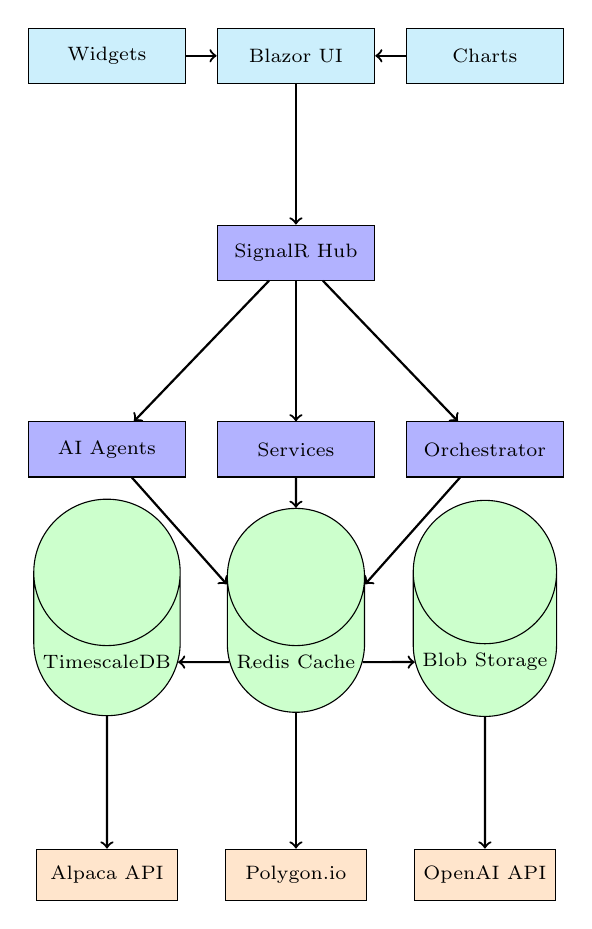
\begin{tikzpicture}[scale=0.42, node distance=1.5cm,
    frontend/.style={rectangle, draw, fill=cyan!20, minimum width=2.0cm, minimum height=0.7cm, text centered, font=\scriptsize},
    backend/.style={rectangle, draw, fill=blue!30, minimum width=2.0cm, minimum height=0.7cm, text centered, font=\scriptsize},
    data/.style={cylinder, draw, fill=green!20, minimum width=1.7cm, minimum height=0.65cm, font=\scriptsize, shape border rotate=90},
    external/.style={rectangle, draw, fill=orange!20, minimum width=1.8cm, minimum height=0.65cm, text centered, font=\scriptsize}]

% Frontend layer
\node[frontend] (blazor) {Blazor UI};
\node[frontend, left of=blazor, node distance=2.4cm] (widgets) {Widgets};
\node[frontend, right of=blazor, node distance=2.4cm] (charts) {Charts};

% SignalR layer
\node[backend, below of=blazor, yshift=-1.0cm] (signalr) {SignalR Hub};

% Backend services
\node[backend, below of=signalr, yshift=-1.0cm, xshift=-2.4cm] (agents) {AI Agents};
\node[backend, below of=signalr, yshift=-1.0cm] (services) {Services};
\node[backend, below of=signalr, yshift=-1.0cm, xshift=2.4cm] (orchestrator) {Orchestrator};

% Data layer
\node[data, below of=services, yshift=-1.2cm] (cache) {Redis Cache};
\node[data, left of=cache, node distance=2.4cm] (timeseries) {TimescaleDB};
\node[data, right of=cache, node distance=2.4cm] (blob) {Blob Storage};

% External APIs
\node[external, below of=timeseries, yshift=-1.2cm] (alpaca) {Alpaca API};
\node[external, below of=cache, yshift=-1.2cm] (polygon) {Polygon.io};
\node[external, below of=blob, yshift=-1.2cm] (openai) {OpenAI API};

% Connections
\draw[->, thick] (widgets) -- (blazor);
\draw[->, thick] (charts) -- (blazor);
\draw[->, thick] (blazor) -- (signalr);
\draw[->, thick] (signalr) -- (agents);
\draw[->, thick] (signalr) -- (services);
\draw[->, thick] (signalr) -- (orchestrator);
\draw[->, thick] (agents) -- (cache);
\draw[->, thick] (services) -- (cache);
\draw[->, thick] (orchestrator) -- (cache);
\draw[->, thick] (cache) -- (timeseries);
\draw[->, thick] (cache) -- (blob);
\draw[->, thick] (timeseries) -- (alpaca);
\draw[->, thick] (cache) -- (polygon);
\draw[->, thick] (blob) -- (openai);

\end{tikzpicture}
\caption{Production Web Architecture: Real-time Blazor dashboard with SignalR streaming and distributed caching}
\label{fig:web-architecture}
\end{figure}

\subsubsection{Scalability and Performance}

\textbf{Production-Grade Infrastructure}

FeenQR is designed for enterprise deployment with scalability features:

\begin{itemize}
    \item \textbf{Distributed Caching}: Redis for high-speed data access
    \item \textbf{Time Series Database}: TimescaleDB for efficient historical data storage
    \item \textbf{Async/Await Patterns}: Non-blocking I/O throughout the codebase
    \item \textbf{Connection Pooling}: Optimized database and API connections
    \item \textbf{Rate Limiting}: Intelligent API quota management
    \item \textbf{Circuit Breakers}: Fault tolerance for external service failures
    \item \textbf{Horizontal Scaling}: Containerized deployment with Kubernetes support
\end{itemize}

\section{Future Enhancements}

\subsection{Phase 1: Core Statistical Framework (Completed)}
\textbf{Status}: Implemented

Delivered comprehensive statistical capabilities:
\begin{itemize}
    \item Statistical hypothesis testing suite (t-tests, ANOVA, chi-square)
    \item Time series analysis (stationarity, autocorrelation, seasonal decomposition)
    \item Cointegration analysis (Engle-Granger, Johansen tests)
    \item Power analysis and sample size calculations
\end{itemize}

\subsection{Phase 2: Machine Learning and Predictive Modeling (Completed)}
\textbf{Status}: Implemented

Advanced ML capabilities delivered:
\begin{itemize}
    \item Time series forecasting (ARIMA/SARIMA, exponential smoothing)
    \item Feature engineering pipeline (technical indicators, lagged variables)
    \item Model validation framework (cross-validation, walk-forward analysis)
    \item Prophet integration for advanced forecasting
\end{itemize}

\subsection{Phase 3: Advanced Analytics and Risk Management (In Progress)}
\textbf{Status}: Partially Implemented

Currently developing:
\begin{itemize}
    \item Factor modeling and risk decomposition
    \item Advanced optimization algorithms
    \item High-frequency trading capabilities
    \item Real-time risk monitoring systems
\end{itemize}

\subsection{Phase 4: Web Interface Transformation (In Progress)}
\textbf{Status}: Active Development

Bloomberg Terminal-style web application:
\begin{itemize}
    \item Multi-widget dashboard interface
    \item Real-time data streaming via SignalR
    \item Professional UI components (MudBlazor/Radzen)
    \item Drag-and-drop widget management
    \item Dark theme and keyboard shortcuts
\end{itemize}

\subsection{Phase 5: Enterprise Features (Planned)}
\textbf{Status}: Planned

Future enterprise capabilities:
\begin{itemize}
    \item Multi-user collaboration platform
    \item Advanced compliance and audit trails
    \item Cloud-native deployment (Azure/AWS)
    \item API gateway and microservices architecture
    \item Advanced security and access control
\end{itemize}

\section{Limitations and Challenges}

\subsection{Technical Limitations}

\subsubsection{Performance Constraints}
\begin{itemize}
    \item \textbf{Memory Usage}: Large datasets require significant RAM for analysis
    \item \textbf{Processing Speed}: Complex ML models may require optimization for real-time use
    \item \textbf{Database Scalability}: Current architecture may need optimization for high-frequency data
    \item \textbf{Network Dependencies}: Heavy reliance on external API availability
\end{itemize}

\subsubsection{Platform Dependencies}
\begin{itemize}
    \item \textbf{.NET Ecosystem}: Limited to Windows/.NET environments (though .NET 9.0 improves cross-platform)
    \item \textbf{External APIs}: Dependent on third-party service availability and rate limits
    \item \textbf{Data Quality}: Analysis quality depends on input data accuracy and completeness
\end{itemize}

\subsection{Operational Challenges}

\subsubsection{Data Integration Complexity}
\begin{itemize}
    \item \textbf{API Rate Limiting}: External data providers impose usage restrictions
    \item \textbf{Data Synchronization}: Maintaining consistency across multiple data sources
    \item \textbf{Real-Time Processing}: Balancing analysis depth with latency requirements
\end{itemize}

\subsubsection{AI and ML Limitations}
\begin{itemize}
    \item \textbf{Model Accuracy}: AI predictions are probabilistic and require validation
    \item \textbf{Overfitting Risk}: ML models may perform well in backtesting but fail in live markets
    \item \textbf{Interpretability}: Complex models may lack transparency in decision-making
\end{itemize}

\subsection{Regulatory and Compliance Considerations}

\subsubsection{Financial Regulation}
\begin{itemize}
    \item \textbf{SEC Compliance}: Automated trading systems require regulatory approval
    \item \textbf{Risk Disclosure}: AI-driven strategies need clear risk communication
    \item \textbf{Audit Trails}: Comprehensive logging required for regulatory compliance
\end{itemize}

\subsubsection{Data Privacy}
\begin{itemize}
    \item \textbf{Personal Data Handling}: Compliance with GDPR and privacy regulations
    \item \textbf{Data Security}: Protection of sensitive financial and personal information
    \item \textbf{Third-Party Risk}: Vendor risk assessment for data providers
\end{itemize}

\section{Strengths and Competitive Advantages}

\subsection{Architectural Strengths}

\subsubsection{Modular Plugin Architecture}
\begin{itemize}
    \item \textbf{Extensibility}: Easy addition of new analysis capabilities
    \item \textbf{Maintainability}: Isolated components reduce system complexity
    \item \textbf{Scalability}: Independent scaling of different analysis modules
    \item \textbf{Reusability}: Plugin reuse across different research workflows
\end{itemize}

\subsubsection{AI-First Design}
\begin{itemize}
    \item \textbf{Natural Language Interface}: Conversational research interactions
    \item \textbf{Autonomous Operation}: Self-managing agent workflows
    \item \textbf{Adaptive Learning}: Performance-based strategy adjustment
    \item \textbf{Multi-Modal Processing}: Text, audio, numerical, and visual data analysis
\end{itemize}

\subsection{Market Differentiation}

\subsubsection{Comprehensive Data Integration}
\begin{itemize}
    \item \textbf{Multi-Source Analysis}: Unified processing of traditional and alternative data
    \item \textbf{Real-Time Processing}: Live data integration with analysis capabilities
    \item \textbf{Historical Depth}: Extensive historical data for backtesting and validation
\end{itemize}

\subsubsection{Research Automation}
\begin{itemize}
    \item \textbf{Workflow Orchestration}: Automated research pipeline execution
    \item \textbf{Signal Generation}: AI-driven trading signal creation and validation
    \item \textbf{Risk Integration}: Embedded risk management throughout research process
\end{itemize}

\subsection{Technology Advantages}

\subsubsection{Semantic Kernel Integration}
\begin{itemize}
    \item \textbf{Advanced AI Orchestration}: Sophisticated agent coordination
    \item \textbf{Plugin Ecosystem}: Rich library of AI-powered functions
    \item \textbf{Natural Language Processing}: Advanced content understanding
    \item \textbf{Function Calling}: Structured AI-system interactions
\end{itemize}

\subsubsection{Modern Technology Stack}
\begin{itemize}
    \item \textbf{.NET 9.0}: Latest runtime with performance and security improvements
    \item \textbf{Cross-Platform}: Deployment flexibility across operating systems
    \item \textbf{Type Safety}: Compile-time error prevention and code reliability
    \item \textbf{Performance}: High-performance computing capabilities
\end{itemize}

\section{Industrial Adoption Assessment}

\subsection{Technology Readiness Level (TRL)}
\textbf{Current TRL: 7-8 (System Prototype to System Complete)}

\subsubsection{TRL 7: System Prototype Demonstration}
\begin{itemize}
    \item \textbf{Validated}: Core functionality demonstrated in operational environment
    \item \textbf{Integrated}: All major components working together
    \item \textbf{Representative}: Realistic operational scenarios tested
\end{itemize}

\subsubsection{Approaching TRL 8: System Complete}
\begin{itemize}
    \item \textbf{Performance}: System performance characterized in operational environment
    \item \textbf{Documentation}: Complete technical documentation available
    \item \textbf{Validation}: System validation in relevant operational environment
\end{itemize}

\subsection{Market Readiness Assessment}

\subsubsection{Target Market Segments}
\begin{itemize}
    \item \textbf{Quantitative Hedge Funds}: Advanced research automation needs
    \item \textbf{Asset Management Firms}: Multi-asset portfolio analysis requirements
    \item \textbf{Investment Banks}: Research department productivity enhancement
    \item \textbf{Prop Trading Firms}: High-frequency and algorithmic trading
    \item \textbf{Family Offices}: Comprehensive risk management and analysis
\end{itemize}

\subsubsection{Competitive Positioning}
\begin{itemize}
    \item \textbf{vs. Traditional Platforms}: Excel, MATLAB, R - Superior automation and AI integration
    \item \textbf{vs. Commercial Solutions}: Bloomberg Terminal, FactSet - Cost-effective alternative
    \item \textbf{vs. Open-Source Tools}: QuantConnect, Zipline - More comprehensive AI capabilities
    \item \textbf{vs. Cloud Solutions}: AWS Sagemaker, Google AI Platform - Specialized for finance
\end{itemize}

\subsection{Adoption Barriers and Mitigations}

\subsubsection{Technical Barriers}
\begin{itemize}
    \item \textbf{Complexity}: Steep learning curve for non-technical users
    \item \textbf{Mitigation}: Intuitive web interface and comprehensive documentation
    \item \textbf{Integration}: Compatibility with existing infrastructure
    \item \textbf{Mitigation}: API-first design and standard protocols
\end{itemize}

\subsubsection{Organizational Barriers}
\begin{itemize}
    \item \textbf{Cultural Resistance}: Resistance to AI-driven decision making
    \item \textbf{Mitigation}: Transparent AI explanations and human oversight capabilities
    \item \textbf{Regulatory Uncertainty}: Evolving AI regulation in finance
    \item \textbf{Mitigation}: Compliance-first architecture and audit trails
\end{itemize}

\subsubsection{Financial Barriers}
\begin{itemize}
    \item \textbf{Implementation Cost}: Initial setup and training investment
    \item \textbf{Mitigation}: Phased implementation and clear ROI demonstration
    \item \textbf{API Costs}: External data provider fees
    \item \textbf{Mitigation}: Flexible data source configuration and cost optimization
\end{itemize}

\subsection{Go-to-Market Strategy}

\subsubsection{Phase 1: Beta Program (Q1 2026)}
\begin{itemize}
    \item \textbf{Target}: Early adopter quantitative funds and research firms
    \item \textbf{Value Proposition}: 10x productivity improvement in research workflows
    \item \textbf{Delivery}: Cloud-hosted solution with professional services
\end{itemize}

\subsubsection{Phase 2: Commercial Launch (Q3 2026)}
\begin{itemize}
    \item \textbf{Target}: Mid-tier asset managers and investment banks
    \item \textbf{Value Proposition}: Complete research platform replacement
    \item \textbf{Delivery}: On-premise and cloud deployment options
\end{itemize}

\subsubsection{Phase 3: Enterprise Expansion (Q1 2027)}
\begin{itemize}
    \item \textbf{Target}: Large financial institutions and enterprise clients
    \item \textbf{Value Proposition}: Enterprise-grade compliance and scalability
    \item \textbf{Delivery}: Custom integrations and white-label solutions
\end{itemize}

\section{Implementation Roadmap}

\subsection{Short-Term (0-6 months)}
\begin{itemize}
    \item Complete web interface transformation
    \item Enhance real-time data processing capabilities
    \item Implement advanced compliance and audit features
    \item Expand alternative data integration
\end{itemize}

\subsection{Medium-Term (6-18 months)}
\begin{itemize}
    \item Launch cloud-native deployment options
    \item Develop multi-user collaboration platform
    \item Implement advanced ML model interpretability
    \item Expand regulatory compliance features
\end{itemize}

\subsection{Long-Term (18+ months)}
\begin{itemize}
    \item Enterprise-scale deployment capabilities
    \item Global market expansion
    \item Advanced AI capabilities (reinforcement learning, generative models)
    \item Industry-specific solution customization
\end{itemize}

\section{Conclusion}

FeenQR represents a significant advancement in quantitative finance research platforms, successfully integrating AI-driven analysis with traditional financial methodologies. The system's modular architecture, comprehensive data integration, and autonomous research capabilities position it as a leading solution for modern quantitative finance.

\subsection{Key Achievements}
\begin{itemize}
    \item Successful implementation of AI-orchestrated research workflows
    \item Comprehensive integration of traditional and alternative data sources
    \item Development of sophisticated risk management and analysis tools
    \item Creation of extensible plugin architecture for continuous capability expansion
\end{itemize}

\subsection{Future Outlook}
The system's trajectory toward industrial adoption is strong, with clear pathways for market penetration and enterprise integration. The combination of technical innovation, practical utility, and regulatory compliance positions FeenQR as a transformative force in quantitative finance.

\subsection{Recommendations}
\begin{itemize}
    \item Accelerate web interface development for improved user adoption
    \item Invest in enterprise compliance and security features
    \item Expand partnership ecosystem for data and technology integration
    \item Develop comprehensive training and support infrastructure
\end{itemize}

The successful evolution of FeenQR from a research prototype to an industrial-grade platform demonstrates the viability of AI-first approaches in quantitative finance, setting new standards for research automation and analytical capabilities.

\section{Project Resources and Links}

\subsection{Repository and Documentation}
\begin{itemize}
    \item \textbf{GitHub Repository}: \url{https://github.com/arithmax-research/FeenQR}
    \item \textbf{Documentation}: \url{https://github.com/arithmax-research/FeenQR/wiki}
    \item \textbf{Issue Tracker}: \url{https://github.com/arithmax-research/FeenQR/issues}
    \item \textbf{Release Notes}: \url{https://github.com/arithmax-research/FeenQR/releases}
\end{itemize}

\subsection{Technical Specifications}
\begin{itemize}
    \item \textbf{Framework}: .NET 9.0
    \item \textbf{Language}: C\# 12.0
    \item \textbf{AI Framework}: Microsoft Semantic Kernel 1.25.0
    \item \textbf{License}: MIT License
    \item \textbf{Platform}: Cross-platform (Windows, macOS, Linux)
\end{itemize}

\subsection{API Integrations}
\begin{itemize}
    \item \textbf{Brokerage APIs}: Alpaca Markets, Interactive Brokers (planned)
    \item \textbf{Market Data}: Polygon.io, Yahoo Finance, Alpha Vantage, IEX Cloud
    \item \textbf{News Sources}: Finviz, YFinance News, Reddit, Twitter
    \item \textbf{Economic Data}: FRED, World Bank, IMF, OECD
    \item \textbf{Academic Research}: Semantic Scholar, arXiv, SSRN
\end{itemize}

\subsection{Development Roadmap}
\begin{itemize}
    \item \textbf{Web Interface}: Bloomberg Terminal-style dashboard (Q1 2026)
    \item \textbf{Cloud Deployment}: Azure-native hosting (Q2 2026)
    \item \textbf{Enterprise Features}: Multi-user collaboration (Q3 2026)
    \item \textbf{Advanced AI}: Reinforcement learning integration (Q4 2026)
\end{itemize}

\subsection{Community and Support}
\begin{itemize}
    \item \textbf{Discord Community}: \url{https://discord.gg/arithmax-research}
    \item \textbf{LinkedIn}: \url{https://linkedin.com/company/arithmax-research}
    \item \textbf{Twitter}: \url{https://twitter.com/arithmax_research}
    \item \textbf{Email Support}: support@arithmax.com
\end{itemize}

\begin{thebibliography}{9}
\bibitem{feenqr-repo}
Arithmax Research, ``FeenQR: Intelligent Quantitative Research Agent System,'' 2025. [Online]. Available: https://github.com/arithmax-research/FeenQR

\bibitem{semantic-kernel}
Microsoft, ``Semantic Kernel Documentation,'' 2025. [Online]. Available: https://learn.microsoft.com/en-us/semantic-kernel/

\bibitem{alpaca-markets}
Alpaca, ``Alpaca Markets API Documentation,'' 2025. [Online]. Available: https://alpaca.markets/docs/

\bibitem{mathnet-numerics}
Math.NET, ``Math.NET Numerics Documentation,'' 2025. [Online]. Available: https://numerics.mathdotnet.com/

\bibitem{microsoft-ml}
Microsoft, ``ML.NET Documentation,'' 2025. [Online]. Available: https://dotnet.microsoft.com/en-us/apps/machinelearning-ai/ml-dotnet

\end{thebibliography}

\end{document}